%UCE-3: Aggiunge CRS

\begin{figure}
\centering
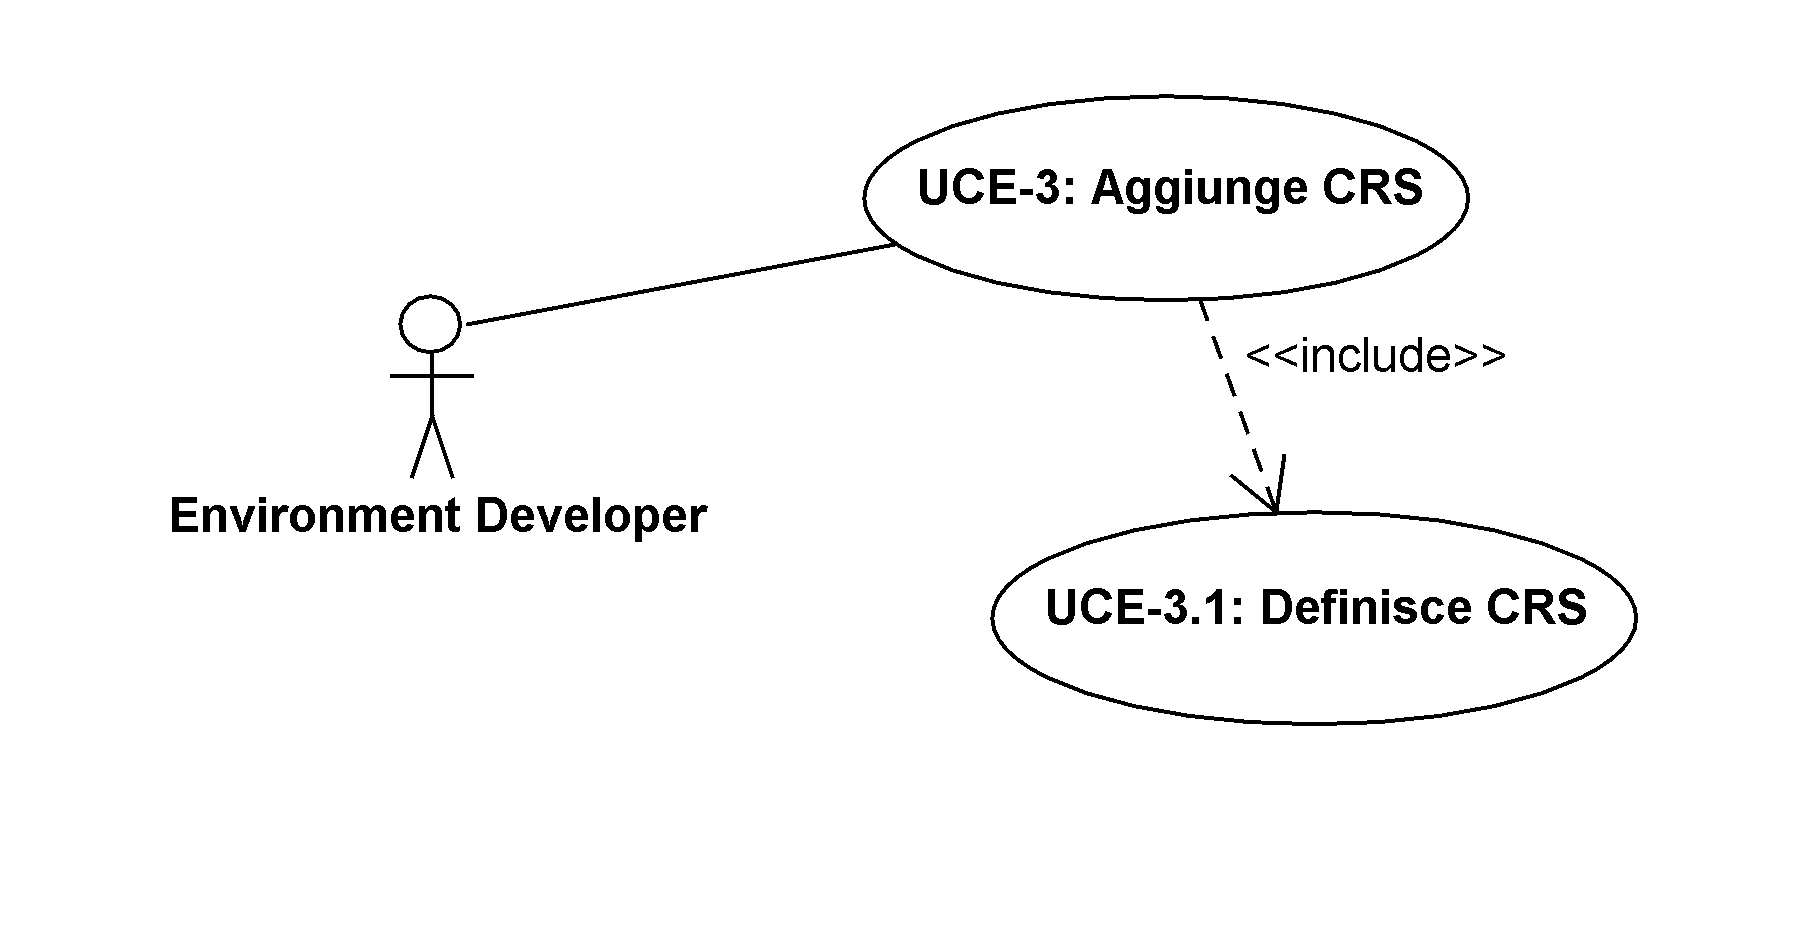
\includegraphics[width=1.1\textwidth]{Immagini/Capitolo2/UseCases/UCE-3.png}
\caption{Diagramma dei casi d'uso UCE-3}\label{fig:uc-uce-3}
\end{figure}


\begin{itemize}
	\item \textbf{Attori:} ED
	\item \textbf{Scopo e descrizione:} l'ED deve essere in grado di definire ed aggiungere una nuova \emph{strategia di risoluzione dei conflitti} (CRS)
	\item \textbf{Pre-condizioni:} il software fornisce meccanismi per la definizione e l'aggiunta di CRS, il sistema non è attivo
	\item \textbf{Post-condizioni:} il sistema è attivo e la una nuova CRS è disponibile
	\item \textbf{Flusso principale degli eventi:}
		\begin{enumerate}
			\item l'ED definisce una nuova CRS attraverso i meccanismi previsti dal sistema (si guardi il caso d'uso \emph{UCE-3.1})
			\item l'ED aggiunge la nuova CRS al sistema
			\item l'ED avvia il sistema
		\end{enumerate}
\end{itemize}


\paragraph{UCE-3.1: Definisce CRS}

\begin{itemize}
	\item \textbf{Attori:} ED
	\item \textbf{Scopo e descrizione:} l'ED deve essere in grado di definire una nuova CRS
	\item \textbf{Pre-condizioni:} il sistema è stato configurato correttamente. Il sistema non è attivo. Il sistema offre meccanismi per la definizione di una nuova CRS.
	\item \textbf{Post-condizioni:} una nuova CRS è disponibile per l'integrazione al sistema
	\item \textbf{Flusso principale degli eventi:}
		\begin{enumerate}
			\item l'ED definisce una nuova CRS
			\item l'ED realizza la CRS in una unità di elaborazione separata e raggiungibile al software
		\end{enumerate}
	
\end{itemize}

